\documentclass{article}

\usepackage{amsmath,amssymb,amsthm}
\usepackage[shortlabels]{enumitem}
\usepackage{tikz}
\usetikzlibrary{automata, arrows.meta, positioning}

\title{Solutions to ``Elements of the Theory of Computation'', 2nd edition
(Lewis, Papadimitriou)}
\author{Ng Wei En}

\begin{document}

\maketitle
\tableofcontents
\newpage

\setcounter{section}{1}
\section{Finite Automata}

\subsection{Deterministic Finite Automata}

\paragraph{2.1.3.}

\begin{enumerate}[(a)]
\item 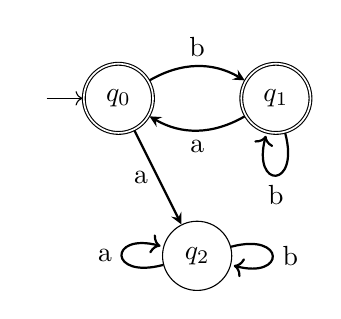
\begin{tikzpicture}[auto]
  \node (q0) [state, initial, accepting, initial text = {}] at (0,0) {$q_0$};
  \node (q1) [state, accepting] at (2,0) {$q_1$};
  \node (q2) [state] at (1,-2) {$q_2$};

  \path [-stealth, thick]
    (q0) edge node [left] {a} (q2)
    (q0) edge [bend left] node {b} (q1)
    (q1) edge [bend left] node {a} (q0)
    (q1) edge [loop below] node {b} ()
    (q2) edge [loop left] node {a} ()
    (q2) edge [loop right] node {b} ();
  \end{tikzpicture}
\item 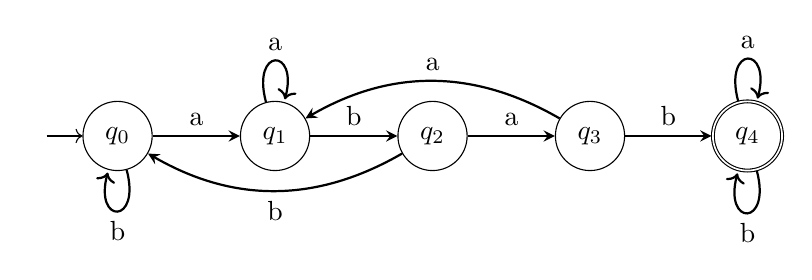
\begin{tikzpicture}[auto]
  \node (q0) [state, initial, initial text = {}] at (0,0) {$q_0$};
  \node (q1) [state] at (2,0) {$q_1$};
  \node (q2) [state] at (4,0) {$q_2$};
  \node (q3) [state] at (6,0) {$q_3$};
  \node (q4) [state, accepting] at (8,0) {$q_4$};

  \path [-stealth, thick]
    (q0) edge node {a} (q1)
    (q0) edge [loop below] node {b} ()
    (q1) edge [loop above] node {a} ()
    (q1) edge node {b} (q2)
    (q2) edge node {a} (q3)
    (q2) edge [bend left] node {b} (q0)
    (q3) edge [bend right] node [above] {a} (q1)
    (q3) edge node {b} (q4)
    (q4) edge [loop above] node {a} ()
    (q4) edge [loop below] node {b} ();
\end{tikzpicture}
\item 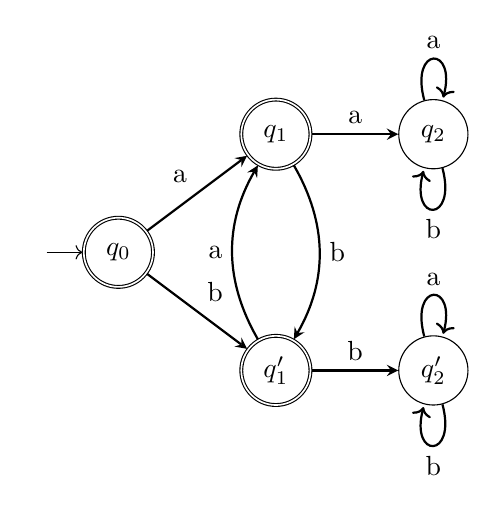
\begin{tikzpicture}[auto]
  \node (q0) [state, initial, accepting, initial text = {}] at (0,-1.5) {$q_0$};
  \node (q1) [state, accepting] at (2,0) {$q_1$};
  \node (q2) [state] at (4,0) {$q_2$};
  \node (q1') [state, accepting] at (2,-3) {$q_1'$};
  \node (q2') [state] at (4,-3) {$q_2'$};

  \path [-stealth, thick]
    (q0) edge node {a} (q1)
    (q0) edge node {b} (q1')
    (q1) edge node {a} (q2)
    (q1) edge [bend left] node {b} (q1')
    (q2) edge [loop above] node {a} ()
    (q2) edge [loop below] node {b} ()
    (q1') edge [bend left] node {a} (q1)
    (q1') edge node {b} (q2')
    (q2') edge [loop above] node {a} ()
    (q2') edge [loop below] node {b} ();
\end{tikzpicture}
\item 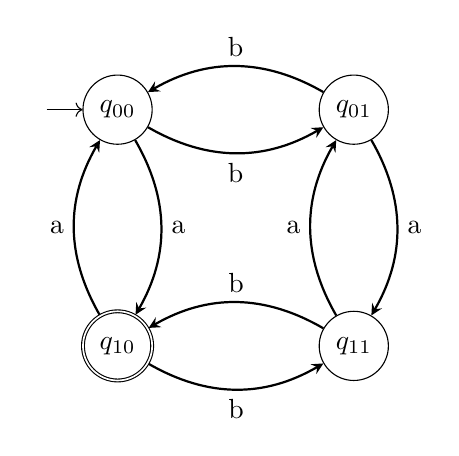
\begin{tikzpicture}[auto]
  \node (q00) [state, initial, initial text = {}] at (0,0) {$q_{00}$};
  \node (q01) [state] at (3,0) {$q_{01}$};
  \node (q10) [state, accepting] at (0,-3) {$q_{10}$};
  \node (q11) [state] at (3,-3) {$q_{11}$};

  \path [-stealth, thick]
    (q00) edge [bend left] node {a} (q10)
    (q00) edge [bend right] node [below] {b} (q01)
    (q01) edge [bend left] node {a} (q11)
    (q01) edge [bend right] node [above] {b} (q00)
    (q10) edge [bend left] node {a} (q00)
    (q10) edge [bend right] node [below] {b} (q11)
    (q11) edge [bend left] node {a} (q01)
    (q11) edge [bend right] node [above] {b} (q10);
\end{tikzpicture}
\item 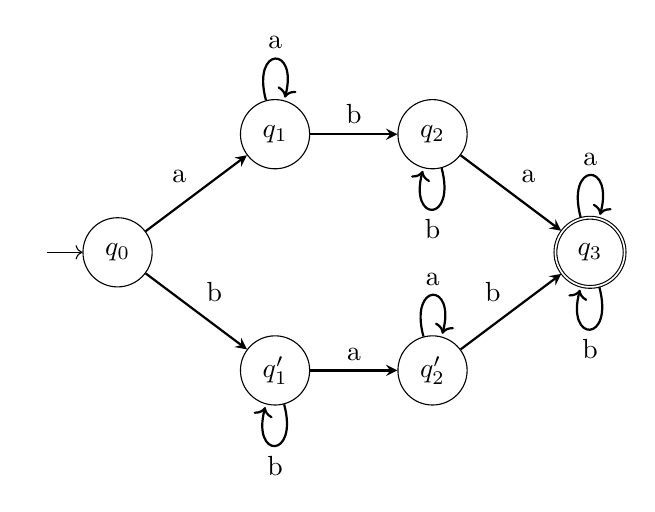
\begin{tikzpicture}[auto]
  \node (q0) [state, initial, initial text = {}] at (0,-1.5) {$q_0$};
  \node (q1) [state] at (2, 0) {$q_1$};
  \node (q2) [state] at (4, 0) {$q_2$};
  \node (q3) [state, accepting] at (6,-1.5) {$q_3$};
  \node (q1') [state] at (2, -3) {$q_1'$};
  \node (q2') [state] at (4, -3) {$q_2'$};

  \path [-stealth, thick]
    (q0) edge node {a} (q1)
    (q0) edge node {b} (q1')
    (q1) edge [loop above] node {a} ()
    (q1) edge node {b} (q2)
    (q2) edge node {a} (q3)
    (q2) edge [loop below] node {b} ()
    (q3) edge [loop above] node {a} ()
    (q3) edge [loop below] node {b} ()
    (q1') edge node {a} (q2')
    (q1') edge [loop below] node {b} ()
    (q2') edge [loop above] node {a} ()
    (q2') edge node {b} (q3);
\end{tikzpicture}
\end{enumerate}

\paragraph{2.1.4.}
\begin{enumerate}[(a)]
\item \begin{enumerate}[(i)]
  \item 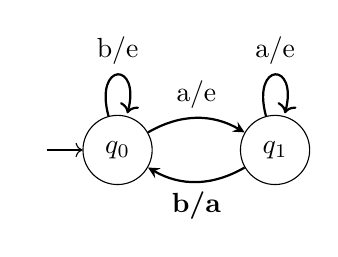
\begin{tikzpicture}[auto]
    \node (q0) [state, initial, initial text = {}] at (0,0) {$q_0$};
    \node (q1) [state] at (2,0) {$q_1$};

    \path [-stealth, thick]
      (q0) edge [bend left] node {a/e} (q1)
      (q0) edge [loop above] node {b/e} ()
      (q1) edge [loop above] node {a/e} ()
      (q1) edge [bend left] node {\textbf{b/a}} (q0);
    \end{tikzpicture}
  \item 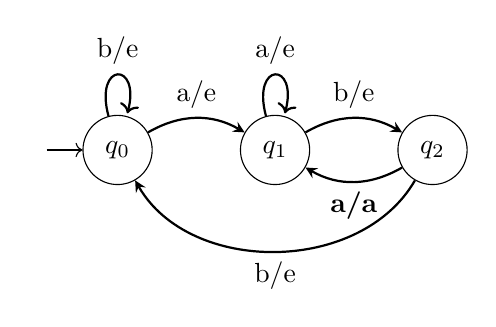
\begin{tikzpicture}[auto]
    \node (q0) [state, initial, initial text = {}] at (0,0) {$q_0$};
    \node (q1) [state] at (2,0) {$q_1$};
    \node (q2) [state] at (4,0) {$q_2$};

    \path [-stealth, thick]
      (q0) edge [bend left] node {a/e} (q1)
      (q0) edge [loop above] node {b/e} ()
      (q1) edge [loop above] node {a/e} ()
      (q1) edge [bend left] node {b/e} (q2)
      (q2) edge [bend left] node {\textbf{a/a}} (q1)
      (q2) edge [bend left=60] node {b/e} (q0);
    \end{tikzpicture}
  \item 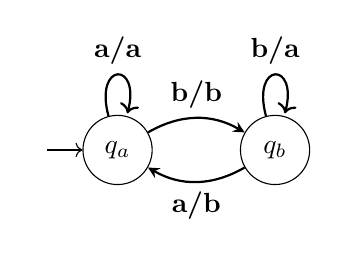
\begin{tikzpicture}[auto]
    \node (qa) [state, initial, initial text = {}] at (0,0) {$q_a$};
    \node (qb) [state] at (2,0) {$q_b$};

    \path [-stealth, thick]
      (qa) edge [loop above] node {\textbf{a/a}} (qa)
      (qa) edge [bend left] node {\textbf{b/b}} (qb)
      (qb) edge [bend left] node {\textbf{a/b}} (qa)
      (qb) edge [loop above] node {\textbf{b/a}} ();
    \end{tikzpicture}
  \end{enumerate}
\item \begin{enumerate}[(i)]
  \item A \textbf{deterministic finite-state transducer} is a quintuple $T = (K,
    \Sigma, \delta, s, L)$ where \begin{itemize}[label={}]
    \item $K$ is a finite set of \textbf{states},
    \item $\Sigma$ is an alphabet,
    \item $s \in K$ is the \textbf{initial state},
    \item $L \in \Sigma^*$ is the \textbf{output string}, and
    \item $\delta$, the \textbf{transition function}, is a function from $K
      \times \Sigma$ to $K \times \Sigma^*$.
    \end{itemize}
  \end{enumerate}
  \item A \textbf{configuration of a deterministic finite-state transducer} is
    any element of $K \times \Sigma^* \times \Sigma^*$.
  \item If $(q, w, l)$ and $(q', w', l')$ are two configurations of $T$, then
    $(q, w, l) \vdash_T (q', w', l')$ if and only if $w = aw'$ for some symbol
    $a \in \Sigma$, $l' = lb$ for some string $b \in \Sigma^*$, and
    $\delta(q, a) = (q', b)$.
  \item Denote the reflexive, transitive closure of $\vdash_T$ by $\vdash_T^*$;
    $T$ produces output $u$ on input $w$ if and only if $(s, w, e) \vdash_T^*
    (q, e, u)$ for some $q \in K$.
  \item $T$ computes some function $f: \Sigma^* \to \Sigma^*$, \[
      f(w) = u \iff T\text{ produces output }u\text{ on input }w.
    \]
\end{enumerate}

\end{document}
